\section{A New Design for Secure Virtualization Systems}
\label{sec.design}

%Providing essential system functionality without exposing privileged code is a
%critical challenge in the design of secure systems.
%Currently, there are two basic approaches.
%One, known as system call interposition (SCI), checks and passes system calls
%through to the underlying kernel. The other, which we call ``functionality
%re-creation," requires rebuilding system functionality with new code. In this
%section, we show that both existing methods are limited in their ability to
%prevent attacks in the kernel.
%Using our metric described in Section~\ref{sec.metric},
%we then propose a new design scheme named \lip, which accesses only popular
%code paths through a very small trusted computing base, and utilizes
%functionality re-creation within a secure sandboxed environment for complex implementations.

In the previous section we have demonstrated that ``popular paths'' correlates statistically-significantly with security. 
Next, we want to demonstrate that our ``popular paths'' metric is useful in devising a feasible design solution to build 
secure virtualization systems. We first briefly discuss the limitations faced by existing methods, due to the lack of a good 
security metric. We then propose our new design scheme named \lip, which accesses only popular code paths. 

\subsection{Previous Attempts and Their Limitations}

\subsubsection{System Call Interposition (SCI)}
SCI systems~\cite{Janus0:96, Janus:99} filter system calls to mediate requests
from untrusted user code instead of allowing it to go directly to the kernel.
The filter checks a predefined security policy to decide which system calls are
allowed to pass to the underlying kernel, and which ones must be stopped.
%Figure \ref{fig:design_system_call_interposition} illustrates how
%system call interposition works. System administrators have direct access to a policy engine that sets and changes security policies.

%\begin{figure}%[h]
%\centering
%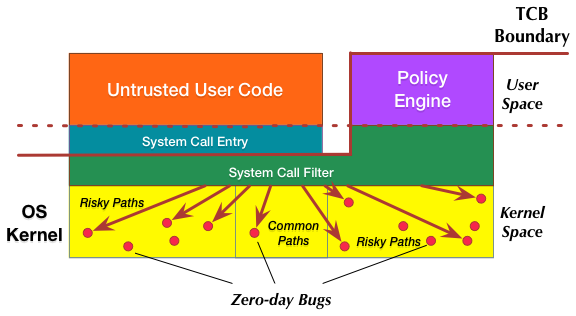
\includegraphics[width=1.0\columnwidth]{diagram/Virtualization_Design_Model_03.png}
%\caption{\small Schematic of how System Call Interposition functions.}
%\label{fig:design_system_call_interposition}
%\end{figure}

%SCI was once popular
%approach to the design of secure virtualization systems because
%because it gave developers the ability to set and enforce security policies.
%\lois{I think I asked this during the last revision. You say ``was"
%a popular approach. Is it not a popular approach anymore?}
%\yiwen{It is not a popular approach anymore, since no modern design could simply rely on
%this idea to build practical system.}
This design is limited by its overly complicated approach to policy
decisions and implementation.
To make a policy decision, the system needs to
obtain and interpret the OS state (e.g., permissions, user groups, register flags)
associated with the programs it is monitoring.
The complexity of OS states makes this process difficult and can lead to
inaccurate policy decisions.
%In addition, there are many indirect paths in the kernel that can be accessed.
%If security policy makers overlook those paths, it renders the
%policy ineffective, as attackers will be able to
%bypass security checks.
%Moreover, blocking
%certain system calls could affect necessary functionality.
%It is difficult for developers to fully understand the side-effects of all the
%system calls in an interface as complex as the UNIX API.
%For example, many applications that rely on \texttt{setuid} fail to check its return value.
%If \texttt{setuid} fails, these applications will continue to function in a compromised state,
%with incorrect permissions and privileges.
%The above limitations make it very challenging to design and build a secure virtualization system using
%system call interposition alone.
%More importantly, there is not a good security metric to indicate if a set of policy decisions is good. 

\subsubsection{Functionality Re-Creation}
Systems such as Drawbridge \cite{Drawbridge-11},
Bascule \cite{Bascule}, and Graphene \cite{Graphene-14} can
provide richer functionality and run more complex programs than most systems built
with SCI alone because they have their own
interfaces and libraries. We label such a design
as ``functionality re-creation."

%\begin{figure}%[h]
%\centering
%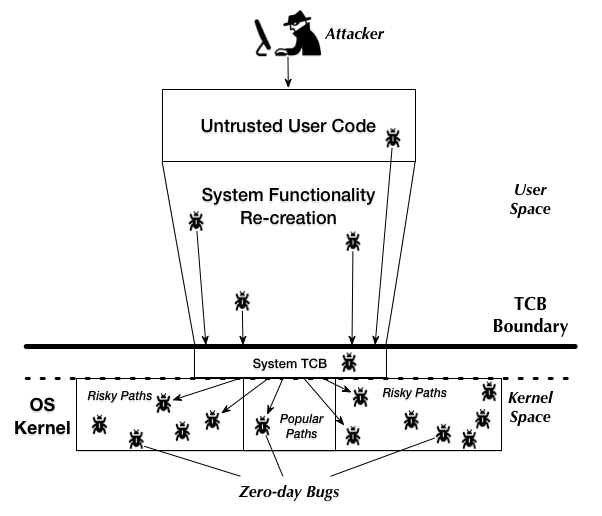
\includegraphics[width=1.0\columnwidth]{diagram/Virtualization_Design_Model_02.png}
%\caption{\small Schematic of a Functionality Re-creation System.}
%\label{fig:design_functionality_reimplementation}
%\end{figure}

The key to this design is to not fully rely on the underlying
kernel for system functions. 
%As illustrated in Figure \ref{fig:design_functionality_reimplementation},
This design re-creates its own system functionalities to provide to user code.
When it has to %communicate with the kernel to
access resources like memory, CPU, and disk storage, the system accesses the kernel directly with
its underlying TCB code.
%which can access the kernel directly.
For example, Graphene \cite{Graphene-14} re-creates its own Linux system calls
in \texttt{libLinux.so}. When it needs to acquire resources from the kernel, it
uses a Platform Adaptation Layer (PAL) with access to the kernel, and provides
basic API functions to the OS library.

Functionality re-creation provides a more realistic solution to building
virtualization systems than earlier efforts.
However, functionality re-creation has two pitfalls: 
first, if the re-created functionality resides in the TCB of the virtualization system, then vulnerabilities there can expose the host OS to attack as well.
For example, hundreds of vulnerabilities have been
reported in existing virtualization systems such as QEMU and VMWare over the past ten years~\cite{NVD}.
In addition, the
complex semantics of OS functions can easily lead to the emergence of bugs during
the re-creation process. Some of these vulnerabilities
can directly lead to privilege escalation, which allows attackers to escape the sandbox
and execute arbitrary code on the host OS.
For example, a vulnerability in VMWare's codebase caused by buffer overflows in the VIX
API allowed local users to
gain privilege to execute arbitrary code in the host
OS~\cite{CVE-2008-2100}.

Second, functionality re-creation may assume that the underlying host kernel is correct. 
As we have seen, this assumption is often incorrect; host kernels may have bugs in their implementation that leave them vulnerable to attack. 
Thus, to provide the greatest assurance that the host kernel will not be exposed to malicious user programs, 
a secure functionality re-creation design should try to deliberately avoid kernel paths that are likely to contain flaws. 
We discuss this approach in detail next.

\subsection{Lock-in-Pop: Staying on the Beaten Path}

As discussed above, a weakness of the previous approaches is the inevitable contact
between the privileged kernel code and an untrusted application.
By leveraging our key metric
that ``popular kernel paths contain fewer bugs," we propose a design
in which all code, including the complex part
of the operating system interface, access only
popular kernel paths through a small TCB. As it ``locks" all functionality
requests into only the ``popular" paths, we dubbed the
design \lip.

\begin{figure}%[h]
\centering
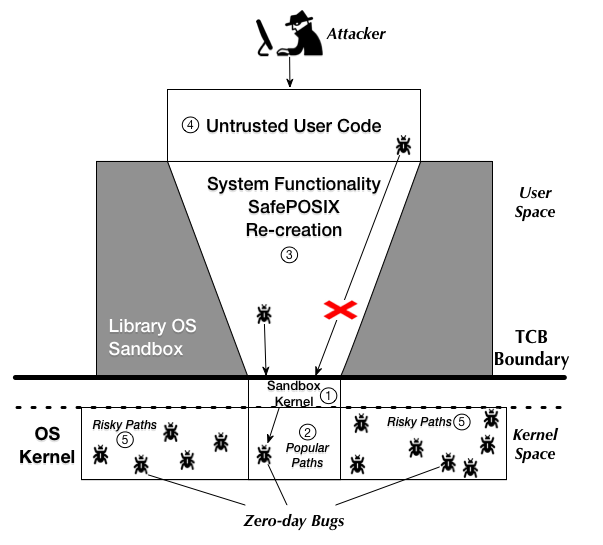
\includegraphics[width=1.0\columnwidth]{diagram/Virtualization_Design_Model_01.png}
\caption{\small \lip design ensures safe execution of untrusted user code
despite existing potential zero-day bugs in the OS kernel.}
\label{fig:design_safe_reimplementation}
\end{figure}

At the lowest level of the design (interfacing with the host OS) is the
sandbox kernel (\ding{172} in Figure \ref{fig:design_safe_reimplementation}).
The sandbox kernel's main role is to ensure that only popular paths (\ding{173} in Figure \ref{fig:design_safe_reimplementation})
of the host OS's kernel can be accessed.
The sandbox kernel could thus function as a very granular system call filter, or
as the core of a programming language sandbox. Note that the functionality
provided by the sandbox kernel is (intentionally) much less than what
an application needs. For example, an application may store files in directories and set permissions on those files.
The sandbox kernel may provide a much simpler abstraction (e.g., a block storage abstraction),
so long as the strictly needed functionality (e.g., persistent storage) is provided.

The application is provided more complex functionality due to the SafePOSIX re-creation
(\ding{174} in Figure \ref{fig:design_safe_reimplementation}).
SafePOSIX has the needed complexity to build the more convenient higher-level
abstractions using the basic functionality the sandbox kernel provides.
The SafePOSIX re-creation is itself isolated within a library OS sandbox, which
forces all system calls from through the sandbox kernel.
So long as this is performed, all calls from SafePOSIX re-creation will only touch the permitted (popular) kernel paths in the underlying host OS.

Similarly, untrusted user code (\ding{175} in Figure \ref{fig:design_safe_reimplementation}) also must be restricted in the way
in which it performs system calls.
System calls must go through the SafePOSIX re-creation, into the sandbox kernel, and then to the host OS.
This is done because if user code could directly make system calls, it could access any paths in the host OS's kernel desired
and thus exploit bugs within them.

Note that it is expected that bugs will occur in many components.
We expect that bugs will occur in the non-popular (risky) kernel paths (\ding{176} in Figure \ref{fig:design_safe_reimplementation}),
bugs will exist in the SafePOSIX re-creation, and the user program will be buggy or even explicitly malicious (created by attackers).
Since the remaining components (\ding{172} and \ding{173} in Figure \ref{fig:design_safe_reimplementation})
are small and/or well tested, this leads to a lower risk of compromise.

\subsection{Implementation of Lock-in-Pop}

To test our \lip design, we used it to implement a prototype virtual machine
called Lind\footnote{\scriptsize Lind is an old English word for a lightweight, but still strong shield
constructed from two layers of linden wood.}. The purpose of building the Lind prototype is to demonstrate that 
our ``popular paths'' metric is practical. And it is indeed possible for developers to build secure systems using 
``popular paths''. 
Lind is divided into a \emph{computational module} that enforces software fault isolation (SFI) and a
\emph{SafePOSIX module} that safely re-creates OS functionality needed by user
applications.  We use a slightly modified version of Native Client
(NaCl)~\cite{NaCl-09} for the computational module; the SafePOSIX is
implemented using Restricted Python (Repy)~\cite{Repy-10}, to support
complex user applications without exposing potentially risky kernel paths.

In this section we provide a brief description of these components and how they
were integrated into Lind, followed by an example of how the system works.

\subsubsection{Primary Components}

\paragraph{Native Client.}
We use NaCl to isolate the computation of the user application
from the kernel. NaCl allows Lind to work on most types of legacy code.
It compiles the programs to produce a binary with software fault isolation.
This prevents applications from performing system calls
or executing arbitrary instructions.
Instead, the application will call into a small, privileged
part of NaCl that forwards system calls. In NaCl's original implementation,
these calls would usually be forwarded to the host OS kernel. In Lind, we
modified NaCl to instead forward these calls to our SafePOSIX re-creation 
(described in detail below).

\paragraph{SafePOSIX.}

To build an API that can access the safe parts of the underlying kernel while
still supporting existing applications, we need two things. First, we need a
restricted sandbox that only allows access to commonly-used kernel paths. We
used Seattle's Repy~\cite{Repy-10} sandbox to perform this task. Second, we
have to provide complex system functions to user programs,
for which we implemented the widely accepted standard POSIX interface on top of Repy, 
which we call SafePOSIX. 

Because the sandbox kernel is the only code that will be in direct contact with host
system calls, it should be small (to make it easy to audit), while providing
primitives that can be used to build more complex functionality.
We used Seattle's Repy system API due to its tiny (around 8K LOC) sandbox
kernel, and its minimal set of system call APIs needed to build general
computational functionality. Repy allows access only to the popular portions of
the OS kernel through 33 basic API functions, including 13 network functions, 6
file functions, 6 threading functions, and 8 miscellaneous functions (Table
\ref{table:RepyKernel})~\cite{Repy-10, RepyKernel}.

\begin{table}
\centering
  \begin{tabular}{ | p{2.5cm} | p{4.5cm} |}
  \hline
  \textbf{Repy Function} & \textbf{Available System Calls}  \\ \hline

Networking & \emph{gethostbyname, openconnection, getmyip, socket.send, socket.receive, socket.close,
listenforconnection, tcpserversocket.getconnection, tcpserversocket.close, sendmessage, listenformessage,
udpserversocket.getmessage, and udpserversocket.close.} \\ \hline

File System I/O Operations & \emph{openfile(filename, create), file.close(), file.readat(size limit, offset), file.writeat(data, offset),
listfiles(), and removefile(filename).} \\ \hline

Threading & \emph{createlock, sleep, lock.acquire, lock.release, createthread, and getthreadname.} \\ \hline

Miscellaneous Functions & \emph{getruntime, randombytes, log, exitall, createvirtualnamespace,
virtualnamespace.evaluate, getresources, and getlasterror.}  \\ \hline
    \end{tabular}
    \caption{Repy sandbox kernel functions that support Lind's SafePOSIX re-creation.}
    \label{table:RepyKernel}
\end{table}


\subsubsection{Enhanced Safety in Call Handling with SafePOSIX Re-creation}

The full kernel interface is extremely rich and hard to protect.
The dual sandbox \lip design used to build Lind provides enhanced
safety protection through both isolation and a POSIX interface (SafePOSIX) that
re-creates risky system calls to
provide full-featured API for legacy applications, with minimal impact on the kernel.

In Lind, a system call issued from user code is
received by NaCl, and then redirected to SafePOSIX.
To service a system call in NaCl, a server routine in
Lind marshals its arguments into a text string, and sends the call and the arguments
to SafePOSIX. The SafePOSIX re-creation serves the system call request, marshals the result, and
returns it back to NaCl. Eventually, the result is returned as the appropriate
native type to the calling program.

SafePOSIX is safe because of two design principles.
First, its re-creation only relies on a small set of basic Repy functions (Table \ref{table:RepyKernel}).
Therefore, the interaction with the host OS kernel is strictly controlled.
Second, the SafePOSIX re-creation is run within the Repy programming language sandbox,
which properly isolates any bugs inside SafePOSIX itself.

%We now offer a more detailed example of how SafePOSIX works by reviewing how it re-creates a file system. 
%The core of the SafePOSIX file system is the \texttt{open}, \texttt{close}, \texttt{read}, \texttt{write},
%\texttt{getdents}, \texttt{stat}, \texttt{mkdir} and \texttt{rmdir} system calls.
%These give the program the illusion of a normal file system even though Repy does not allow directories or access to file attributes.

%When Lind starts, the file system does some pre-initialization. Using the Repy API, the SafePOSIX file system reads a file named ``lind.metadata''
%from the local directory. This file contains packed metadata from previous runs of Lind,
%and is loaded into the runtime SafePOSIX file system data structures.
%There are three main data structures: a list of open file handles, a Python dict of inodes and file metadata,
%and a mapping table to go from a file name and path to an inode number.
%All these data structures are stored in memory, and written to disk when they are changed.

%The \texttt{open} system call is the normal starting point for most file system operations.
%Given a path, it will return a file descriptor to perform other operations like \texttt{read} and \texttt{write}.
%When SafePOSIX receives the \texttt{open} system call, it parses the path, and
%traverses the path in the inode lookup table.
%When SafePOSIX finds the file, it uses the Repy \texttt{openfile} call to get the backing file's object.
%It then picks a free entry from the file handle table, and stores a link to the inode and the file object.
%If the \texttt{create} flag is passed, it adds an entry to the inode and inode lookup table, and creates a new backing file.
%The backing files are not named the same as the actual files, but rather just ``linddata.001,'' ``linddata.002,'' etc.
%The simple names for the backing files allow us to store the real file name in the metadata, a
%necessary step because of Repy's strict rules about the content of filenames.
%Finally, the call returns the index into the file handle table or, if an error was encountered, an error number to which the Unix \texttt{errno} value is set.

%Here is another example of how SafePOSIX re-creation would work with the symbolic link function.
%Instead of relying on the underlying kernel to create symbolic links between real files
%in the host file system, SafePOSIX builds and maintains its own metadata to represent a virtual symbolic link
%between files within its system. In this case, if there is a bug in this symbolic link function,
%such as creation of a link with a deleted file, the bug will be contained within the SafePOSIX re-creation.
%As a result, instead of creating a security issue, the application is denied privileged access to the host OS kernel.
%Therefore, attackers will not be able to leverage a bug within the symbolic link function to exploit the host kernel.

%As described in the above example, the SafePOSIX re-creation only uses a few Repy sandbox kernel functions to access the hardware.
%It creates and maintains its own metadata and data structures, using the Repy programming language sandbox.